\documentclass[../main.tex]{subfiles}
\begin{document}
\chapter{Matrices}
\section{Linear Maps}
\begin{definition}[Linear Map]
  Consider two vector spaces $V$ and $W$.
  A \textit{linear map} is a function $T: V \to W$ such that:
  \[
    T(\lambda\vec{x} + \mu\vec{y}) = \lambda T(\vec{x}) + \mu T(\vec{y})
  \]
  for all $\vec{x}, \vec{y} \in V$ and all scalars $\lambda, \mu \in \R \text{ or }\C$ depending on if $V$ and $W$ are real or complex vector spaces.
\end{definition}
\begin{definition}[Domain and Codomain]
  For a linear map $T: V \to W$, $V$ is called the \textit{domain} and $W$ is called the \textit{codomain}.
\end{definition}
\begin{definition}[Image]
  The \textit{image} of a linear map $T$ is:
  \[
    \im T = \{\vec{x}' \in W : \vec{x}' = T(\vec{x}) \text{ for some } \vec{x} \in V\}
  \]
  If $\vec{x}' = T(\vec{x})$ then $\vec{x}'$ is the \textit{image} of $\vec{x}$ under $T$.
\end{definition}
\begin{definition}[Kernel]
  The \textit{kernel} of a linear map $T$ is:
  \[
    \ker T = \{ \vec{x} \in V : T(\vec{x}) = \vec{0}\}
  \]
  If $\vec{x} \in V$ is such that $T(\vec{x}) = \vec{0}$ then we say that $\vec{x}$ belongs to the \textit{kernel} of $T$.
\end{definition}
\begin{proposition}
  For a linear map $T: V \to W$:
  \begin{enumerate}
    \item $\im T$ is a subspace of $W$
    \item $\ker T$ is a subspace of $V$
  \end{enumerate}
\end{proposition}
\begin{proof}
\begin{enumerate}
  \item Let $\vec{u}', \vec{v}' \in \im T$.
    Therefore there exists, $\vec{u}, \vec{v} \in V$ such that $T(\vec{u}) = \vec{u}'$ and $T(\vec{v}) = \vec{v}'$.
    For any scalars $\lambda, \mu$ we have that $\lambda \vec{u} + \mu \vec{v} \in V$ so $T(\lambda \vec{u} + \mu \vec{v}) \in \im T$.
    By linearity, $T(\lambda \vec{u} + \mu \vec{v}) = \lambda \vec{u}' + \mu \vec{v}'$.
    Thus $\lambda \vec{u}' + \mu \vec{v}' \in \im T$ and $\im T \subseteq W$ so $\im T$ is a subspace of $W$.
  \item Let $\vec{u}, \vec{v} \in \ker T$. Therefore $T(\vec{u}) = T(\vec{v}) = \vec{0}$.
    Consider for any scalars $\lambda, \mu$:
    \[
      T(\lambda \vec{u} + \mu \vec{v}) = \lambda T(\vec{u}) + \mu T(\vec{v}) = \vec{0}
    \]
    Thus $\lambda \vec{u} + \mu \vec{v} \in \ker T$ and $\ker T \subseteq V$ so $\ker T$ is a subspace of $V$.
\end{enumerate}
\end{proof}
\begin{definition}[Rank]
  For a linear map $T$ we define the \textit{rank} to be the dimension of the image. That is:
  \[
    \rank T = \dim (\im T)
  \]
\end{definition}
\begin{definition}[Nullity]
  For a linear map $T$ we define the \textit{nullity} to be the dimension of the kernel. That is:
  \[
    \nullity T = \dim (\ker T)
  \]
\end{definition}
\begin{remark}
  If we have a map $T: V \to W$ then $\nullity T = \dim(\ker T) \leq \dim V$ as the kernel is a subspace of $V$ and $\rank T = \dim(\im T) \leq \dim(W)$ as the image is a subspace of $W$.
\end{remark}
\begin{example}
  \begin{enumerate}
    \item \textbf{Zero linear map -} $T: V \to W$ with $\vec{x} \mapsto \vec{0}$.
      Then we have $\im T = \{\vec{0}\}$ and $\ker T = V$.
    \item \textbf{Identity map -} $T: V \to V$ with $\vec{x} \mapsto \vec{x}$.
      Then we have $\im T = V$ and $\ker T = \{\vec{0}\}$.
    \item Consider $T: \R^2 \to \R^2$ and $\vec{x}' = T(\vec{x})$ with:
      \[
        x'_1 = 2x_1 + x_2 \text{ and } x'_2 = x_1 - 3x_2
      \]
      Then:
      \[
        \begin{pmatrix}
        x'_1 \\
        x'_2 \\
        \end{pmatrix} =
        x_1 \begin{pmatrix}
        2 \\
        1 \\
        \end{pmatrix} +
        x_2 \begin{pmatrix}
        1 \\
        -3 \\
        \end{pmatrix}
      \]
      Since $(2, 1)$ and $(1, -3)$ are linearly independent:
      \[
        \im T = \Span\left\{
        \begin{pmatrix}
        2 \\
        1 \\
        \end{pmatrix},
        \begin{pmatrix}
        1 \\
        -3 \\
        \end{pmatrix}
        \right\} =
        \left\{
        \lambda\begin{pmatrix}
        2 \\
        1 \\
        \end{pmatrix} +
        \mu\begin{pmatrix}
        1 \\
        -3 \\
        \end{pmatrix},\ \lambda, \mu \in \
        \right\}
      \]
      Furthermore, $2x_1 + x_2 = 0$ and $x_1 - 3x_2 = 0 \implies x_1 = x_2 = 0$ so:
      \[
        \ker T = \left\{\begin{pmatrix}
        0 \\
        0 \\
        \end{pmatrix}\right\}
      \]
  \end{enumerate}
\end{example}
\subsubsection{Linear Combinations}
Consider linear maps $T, S: V \to W$.
Then $\alpha T + \beta S: V \to W$ is also a linear map defined by:
\[
  (\alpha T + \beta S)(\vec{x}) = \alpha T(\vec{x}) + \beta S(\vec{x})
\]
for $\alpha, \beta \in \R \text{ or } \C$.
\subsubsection{Composition}
Take linear maps $T: V \to W$ and $S: U \to V$.
Then $U \xrightarrow{S} V \xrightarrow{T} W$ so $T \circ S: U \to W$.
This composition is also a linear map, defined by:
\[
  (T \circ S)(\vec{x}) = T(S(\vec{x}))
\]
\begin{theorem}[Rank-nullity Theore]
  For a linear map $T: V \to W$ then:
  \[
    \label{rankNullity}
    \rank T + \nullity T = \dim V
  \]
\end{theorem}
\begin{proof}
\nonexaminable
Let $n$ be $\dim V$ and $m$ be $\nullity T$.
\[
  \nullity T = \dim (\ker T) \leq \dim V \iff m \leq n
\]
So we only need to consider $m \leq n$.
\begin{proofcases}
  \begin{case}{$m = n$}
    Then $\dim(\ker T) = \dim V$ and since $\ker T$ is a subspace of $V$, we must have $\ker T = V$.
    Therefore $\im T = \{\vec{0}\}$.
    So $\rank T + \nullity T = \dim(\im T) + \dim(\ker T) =0 + n = n$.
  \end{case}
  \begin{case}{$m < n$}
    Let $\{\vec{e}_1, \ldots, \vec{e}_m\}$ be a basis of the kernel of T.
    So $T(\vec{e}_i) = \vec{0}$ for all $i = 1, \ldots, m$.
    We can now extend $\{\vec{e}_1, \ldots, \vec{e}_m\}$ to form a basis of $V$.
    Since $\dim V = n$ the basis must have $n$ elements so:
    \[
      \{\vec{e}_1, \ldots, \vec{e}_m, \vec{e}_{m+1}, \ldots, \vec{e}_n\}
    \]
    We now need to show that $B = \{T(\vec{e}_{m + 1}), \ldots, T(\vec{e}_n)\}$ is a basis of $\im T$.
    \begin{enumerate}
      \item
      To show that $B$ spans $\im T$, take an element $\vec{y} \in \im T$.
      Then by definition, there exists $\vec{x} \in V$ such that $T(\vec{x}) = \vec{y}$.
      Since $\vec{x} \in V$, we can write:
      \[
        \vec{x} = \alpha_1 \vec{e}_1 + \cdots + \alpha_n \vec{e}_n
      \]
      Applying $T$ to this yields:
      \begin{align*}
        \vec{y} = T(\vec{x}) &= T(\alpha_1 \vec{e}_1 + \cdots + \alpha_n \vec{e}_n) \\
                             &= \alpha_1 T(\vec{e}_1) + \cdots \alpha_n T(\vec{e}_n) \\
                             &= \alpha_{m + 1} T(\vec{e}_{m + 1}) + \cdots + \alpha_n T(\vec{e}_n)
      \end{align*}
      Therefore, any element in $\im T$ can be written as a linear combination of vectors from $B$, thus $B$ spans $\im T$.
      \item
      To show that $B$ is linearly independent, consider:
      \[
        \alpha_{m + 1} T(\vec{e}_{m+1}) + \cdots + \alpha_n T(\vec{e}_n) = \vec{0}
      \]
      We now need to show that all of the coefficients are 0.
      By linearity we can write this as:
      \[
        T(\underbrace{\alpha_{m + 1}\vec{e}_{m + 1} + \cdots + \alpha_n \vec{e}_n}_{\vec{x}}) = \vec{0}
      \]
      So $\vec{x} \in \ker T$ and the basis of $\ker T$ is $\{\vec{e}_1, \ldots, \vec{e}_n\}$.
      Therefore there exists $\alpha_1, \cdots \alpha_m$ such that:
      \[
        \vec{x} = \alpha_1 \vec{e}_1 + \cdots + \alpha_m \vec{e}_m
      \]
      We can now equate our two expressions for $\vec{x}$ to get:
      \[
        \alpha_1 \vec{e}_1 + \cdots \alpha_m \vec{e}_m - \alpha_{m + 1}\vec{e}_{m + 1} - \cdots - \alpha_n \vec{e}_n = \vec{0}
      \]
      However $\{\vec{e}_1, \ldots, \vec{e}_m, \vec{e}_{m + 1}, \ldots, \vec{e}_n\}$ is a basis of $V$.
      Since the elements of a basis must be linearly independent, all the coefficients must be 0.
      Thus:
      \[
        \alpha_1 = \cdots = \alpha_m = \alpha_{m + 1} = \cdots = \alpha_n = 0
      \]
      So $B$ is linearly independent.
    \end{enumerate}
    Therefore $B$ is a basis of $\im T$ and so $\rank T = \dim(\im T) = n - m$ as $B$ has $n - m$ elements.
    Thus:
    \[
      \rank T + \nullity T = n - m + m = n = \dim V
    \]
  \end{case}
\end{proofcases}
\end{proof}
\begin{example}
  \begin{enumerate}
    \item For the zero map, $\nullity T = \dim V$ and $\rank T = 0$ so $\nullity T + \rank T = \dim V$.
    \item For the identity map, $\rank T = \dim V$ and $\nullity T = 0$ so $\nullity T + \rank T = \dim V$.
  \end{enumerate}
\end{example}
\section{Matrices as Linear Maps}
Let $M$ be a matrix with entries $M_{i j} \in \R$, where $i$ labels rows and $j$ labels columns.
Then the map defined by $T: \R^{n} \to \R^{n}$, $T(\vec{x}) = \vec{x}' = M\vec{x}$ for $\vec{x}, \vec{x}' \in \R^{n}$ with $x'_i = M_{i j}x_j$, is a linear map.
\begin{example}
  Given $n = 2$:
  \[
    M = \begin{pmatrix}
    M_{1 1} & M_{1 2} \\
    M_{2 1} & M_{2 2} \\
    \end{pmatrix}
  \]
  so we have:
  \[
    \begin{pmatrix}
    x'_1 \\
    x'_2 \\
    \end{pmatrix}
    =
    \begin{pmatrix}
    M_{1 1} & M_{1 2} \\
    M_{2 1} & M_{2 2} \\
    \end{pmatrix}
    \begin{pmatrix}
    x_1 \\
    x_2 \\
    \end{pmatrix}
    =
    \begin{pmatrix}
    M_{1 1}x_1 + M_{1 2}x_2 \\
    M_{2 1}x_1 + M_{2 2}x_2 \\
    \end{pmatrix}
  \]
\end{example}
We can also consider the rows and columns of $M$ as vectors in $\R^{n}$.
We can denote the rows as $\vec{R}_i \in \R^{n}$ and the columns as $\vec{C}_i \in \R^{n}$:
\[
  M = \begin{pmatrix}
  \leftarrow \vec{R}_1 \rightarrow \\
  \cdots \\
  \leftarrow \vec{R}_n \rightarrow
  \end{pmatrix}
  =
  \begin{pmatrix}
  \uparrow & & \uparrow  \\
  \vec{C}_1 & \cdots & \vec{C}_n  \\
  \downarrow &  & \downarrow \\
  \end{pmatrix}
\]
The components are then related in the following form:
\[
  M_{i j} = (\vec{C}_j)_i = (\vec{R}_i)_j
\]
If $\{\vec{e}_1, \ldots, \vec{e}_n\}$ is the standard basis of $\R^{n}$:
\[
  \vec{e}_i \mapsto \vec{e}_i' = T(\vec{e}_i) = M\vec{e}_i = \vec{C}_i
\]
That is, multiplying a matrix by the $i$-th element of the standard basis extracts the $i$-th column.
\[
  \begin{pmatrix}
  M_{1 1} & \cdots & M_{1 n} \\
  \vdots & \ddots & \vdots \\
  M_{n 1} & \cdots & M_{m n} \\
  \end{pmatrix}
  \vec{e}_i = \vec{C}_i
\]
Since $T$ is a linear map for any $\vec{x} \in \R^{n}$:
\[
  \vec{x} = \sum_{i} x_i \vec{e}_i \mapsto T\left(\sum_{i} x_i \vec{e}_i \right) = \sum_{i} x_i \vec{C}_i
\]
Thus $\vec{x} \mapsto x_i \vec{C}_i$.
This means the image of $\vec{x}$ under $T$ a linear combination of the columns of the matrix.
Therefore, $\im T = \im M = \Span\{\vec{C}_1, \ldots, \vec{C}_n\}$.

We can also determine the kernel of $T$ using its matrix representation.
Consider an element of the image, $\vec{x}'$, of $\vec{x}$ under $T$:
\[
  x_i' = M_{i j}x_j = (\vec{R}_i)_j x_j = \vec{R}_i \cdot \vec{x}
\]
so
\[
  \vec{x}' = \begin{pmatrix}
  x_i' \\
  \vdots \\
  x_n' \\
  \end{pmatrix}
  =
  \begin{pmatrix}
  \vec{R}_i \cdot x \\
  \vdots \\
  \vec{R}_n \cdot x \\
  \end{pmatrix}
\]
If $\vec{x} \in \ker T$ then $\vec{x}' = \vec{0}$ so $\vec{R}_1 \cdot \vec{x} = \cdots = \vec{R}_n \cdot \vec{x} = 0$.
Therefore the kernel of $T$ is all vectors that are orthogonal to all rows of the matrix:
\[
  \ker T = \ker M = \{\vec{x} \in \R^{n}: \vec{R}_i \cdot \vec{x} = \vec{0},\ \forall i = 1, \ldots n\}
\]
This is a subspace of $\R^{n}$ as a linear combination of such vectors would also satisfy the above property and therefore would also be in the subspace.
\begin{remark}[Summary]
  \begin{itemize}
    \item $\im M$ is the span of the columns of $M$.
    \item $\ker M$ is the subspace orthogonal to all rows of $M$.
  \end{itemize}
\end{remark}
\begin{example}
  \begin{enumerate}
    \item For $T: \R^{n} \to \R^{n}$, the zero map has representation $\vec{x}' = O\vec{x}$ where $O_{ij} = 0\ \forall i, j$.
      This matrix is called the \textit{zero matrix}.
    \item For $T: \R^{n} \to \R^{n}$, the identity map has representation $\vec{x}' = I\vec{x}$ where $I_{i j} = \delta_{i j}$.
      This matrix is called the \textit{identity matrix}.
    \item For $T: \R^3 \to \R^3$, $\vec{x}' = M \vec{x}$ given by:
      \begin{align*}
        x_1' &= 3x_1 + x_2 + 5x_3 \\
        x_2' &= -x_1 + 2x_3 \\
        x_3' &= 2x_1 + x_2 + 3x_3
      \end{align*}
      This can be converted into matrix form:
      \[
        M = \begin{pmatrix}
        3 & 1 & 5 \\
        -1 & 0 & -2 \\
        2 & 1 & 3 \\
        \end{pmatrix}
      \]
      Since $\im(T)$ is the span of the columns:
      \[
        \im T = \Span\{\vec{C}_1, \vec{C}_2, \vec{C}_3\} = \Span\{\vec{C}_1, \vec{C}_2\}
      \]
      As $\vec{C}_3 = 2\vec{C}_1 - \vec{C}_2$.
      Since $\vec{C}_1, \vec{C}_2$ are linearly independent, $\rank T = \dim(\im T) = 2$.
      From \cref{rankNullity} (rank nullity theorem), we expect $\nullity T = 1$.

      To find $\ker T$ we need to find the subspace orthogonal to all rows.
      \[
        \vec{R}_2 \times \vec{R}_3 = \begin{vmatrix}
        \uvec{i} & \uvec{j} & \uvec{k} \\
        -1 & 0 & -2 \\
        2 & 1 & 3 \\
        \end{vmatrix} =
        \begin{pmatrix}
        2 \\
        -1 \\
        -1 \\
        \end{pmatrix}
      \]
      This is also orthogonal to $\vec{R}_1$ thus:
      \[
        \ker T = \ker M = \Span\left\{
        \begin{pmatrix}
        2 \\
        -1 \\
        -1 \\
        \end{pmatrix}\right\}
      \]
      Since this has dimension 1, $\nullity T = 1$, as expected.
  \end{enumerate}
\end{example}
\section{Geometric Examples\texorpdfstring{ in $\R^2$ and $\R^3$}{}}
\subsection{Examples in \texorpdfstring{$\R^2$}{2D}}
\subsubsection{Rotations}
Consider $\theta$ such that $-\pi < \theta \leq \pi$, then a rotation by angle $\theta$ anticlockwise in $\R^2$ can be represented by:
\[
  \Rot(\theta) = \begin{pmatrix}
  \cos \theta & -\sin \theta \\
  \sin \theta & \cos \theta \\
  \end{pmatrix}
\]
Note that $\det(\Rot(\theta)) = \cos^2 \theta + \sin^2 \theta = 1$.
\begin{center}
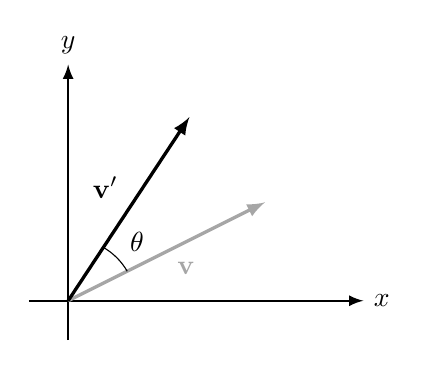
\begin{tikzpicture}[scale=2.5,>=latex]
\draw[->, thick] (-0.2,0) -- (1.5,0) node[right] {$x$};
\draw[->, thick] (0,-0.2) -- (0,1.2) node[above] {$y$};

\coordinate (A) at (1, 0.5);
\coordinate (B) at ({cos(30)*1 - sin(30)*0.5}, {sin(30)*1 + cos(30)*0.5});

\draw[->, very thick, gray!70] (0,0) -- (A) node[midway, below right] {$\mathbf{v}$};

\draw[->, very thick, black] (0,0) -- (B) node[midway, above left] {$\mathbf{v}'$};

\draw[-, black] (0.3,0.15) arc[start angle=30, end angle=60, radius=0.33];
\node at (0.35,0.3) {$\theta$};
\end{tikzpicture}
\end{center}
\subsubsection{Reflections}
Consider $\theta$ such that $-\pi < \theta \leq \pi$, then reflection in the line with angle $\frac{\theta}{2}$ anticlockwise from the $x$-axis (i.e. $y = x\tan(\theta/2)$) in $\R^2$ is represented by:
\[
  \Reflect(\theta) = \begin{pmatrix}
  \cos \theta & \sin \theta \\
  \sin \theta & -\cos \theta \\
  \end{pmatrix}
\]
Note that $\det(\Reflect(\theta)) = -\cos^2 \theta - \sin^2 \theta = -1$.
\begin{center}
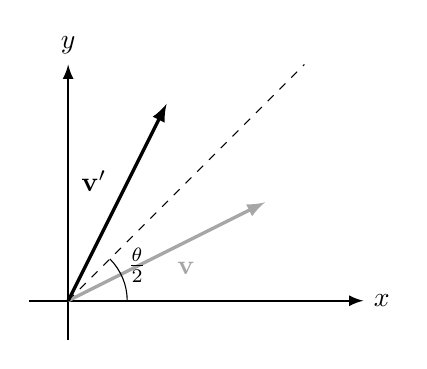
\begin{tikzpicture}[scale=2.5,>=latex]
\draw[->, thick] (-0.2,0) -- (1.5,0) node[right] {$x$};
\draw[->, thick] (0,-0.2) -- (0,1.2) node[above] {$y$};

\coordinate (A) at (1, 0.5);
\coordinate (B) at (0.5, 1);

\draw [black, dashed] (0, 0) -- (1.2, 1.2);
\draw[->, very thick, gray!70] (0,0) -- (A) node[midway, below right] {$\mathbf{v}$};

\draw[->, very thick, black] (0,0) -- (B) node[midway, above left] {$\mathbf{v}'$};

\draw[-, black] (0.3,0) arc[start angle=0, end angle=45, radius=0.3];
\node at (0.35,0.18) {$\frac{\theta}{2}$};
\end{tikzpicture}
\end{center}
\subsubsection{Properties}
\begin{enumerate}
  \item $\Rot(\theta)\Rot(\phi) = \Rot(\theta + \phi)$
  \item $\Reflect(\theta)\Reflect(\phi) = \Rot(\theta - \phi)$
  \item $\Rot(\theta)\Reflect(\phi) = \Reflect(\phi + \theta)$
  \item $\Reflect(\phi)\Rot(\theta) = \Reflect(\phi - \theta)$
\end{enumerate}
\subsection{Examples in \texorpdfstring{$\R^3$}{3D}}
\subsubsection{Rotation along a basis}
Rotation of angle $\theta$ with axis $\vec{e}_1, \vec{e}_2, \vec{e}_3$:
\begin{align*}
  \Rot_{\vec{e}_1}(\theta) &= \begin{pmatrix}
  1 & 0 & 0 \\
  0 & \cos \theta & -\sin \theta \\
  0 & \sin \theta & \cos \theta \\
  \end{pmatrix} \\
  \Rot_{\vec{e}_2}(\theta) &= \begin{pmatrix}
  \cos \theta & 0 & \sin \theta \\
  0 & 1 & 0 \\
  - \sin \theta & 0 & \cos \theta \\
  \end{pmatrix} \\
  \Rot_{\vec{e}_3}(\theta) &= \begin{pmatrix}
  \cos \theta & -\sin \theta & 0 \\
  \sin \theta & \cos \theta & 0 \\
  0 & 0 & 1 \\
  \end{pmatrix}
\end{align*}
\begin{remark}[Warning]
  These look like they all have the same format, however, for $\vec{e}_2$, the negative is on the other $\sin \theta$.
\end{remark}
\subsubsection{Rotation about a unit vector}
Consider a rotation of $\theta$ anticlockwise about a unit vector $\vec{n}$.
For $x \in \R^{3}$
\[
  \vec{x}' = R\vec{x},\ \vec{x}_i' = R_{i j}x_j
\]
We can write:
\[
  \vec{x}' = (\cos \theta)\vec{x} + (1 - \cos \theta)(\vec{n} \cdot \vec{x})\vec{n} + (\sin \theta)(\vec{n} \times \vec{x})
\]
This has matrix representation, $\Rot(\theta, \vec{n})$, given by:
\[
  R_{i j} = \delta_{i j}\cos\theta + (1 - \cos \theta)n_in_j - (\sin \theta)\levi_{i j k}n_k
\]

To show why this is a rotation of $\vec{x}$ about $\vec{n}$, we can first split $\vec{x}$ into a component parallel to $\vec{n}$ and a component perpendicular to $\vec{n}$:
\[
  \vec{x} = \vec{x}_{\parallel} + \vec{x}_{\perp}
\]
where $\vec{x}_{\parallel} = (\vec{x} \cdot \vec{n})\vec{n}$ and $\vec{x}_{\perp}$ such that $\vec{n} \cdot \vec{x}_{\perp} = 0$.

After applying $R$, $\vec{x}_{\parallel}$ is unchanged as it is parallel to the axis of rotation, so $\vec{x}_{\parallel}' = \vec{x}_{\parallel}$.
To find the image of $\vec{x}_{\perp}$, consider the plane passing through the origin orthogonal to $\vec{n}$ and vector $\vec{n} \times \vec{x}$:
\begin{center}
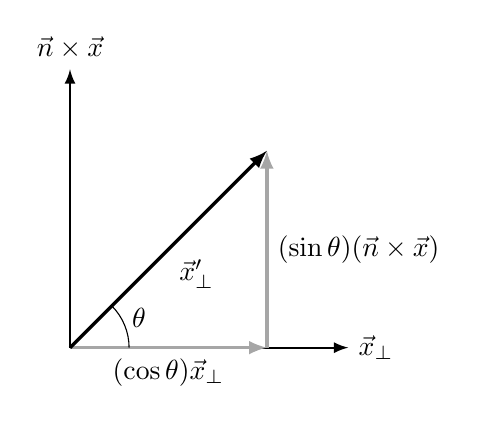
\begin{tikzpicture}[scale=2.5,>=latex]
\draw[->, thick] (0,0) -- (1.414,0) node[right] {$\vec{x}_{\perp}$};
\draw[->, thick] (0,0) -- (0,1.414) node[above] {$\vec{n} \times \vec{x}$};

\draw[->, very thick, gray!70] (1, 0) -- (1, 1) node[midway, right, black] {$(\sin \theta)(\vec{n} \times \vec{x})$};
\draw[->, very thick, gray!70] (0, 0) -- (1, 0) node[midway, below, black] {$(\cos \theta)\vec{x}_{\perp}$};
\draw[->, very thick] (0,0) -- (1,1) node[midway, below right] {$\vec{x}_{\perp}'$};

\draw[black] (0.3,0) arc[start angle=0, end angle=45, radius=0.3];
\node at (0.35,0.15) {$\theta$};
\end{tikzpicture}
\end{center}
We get $(\sin \theta)(\vec{n} \times \vec{x})$ as $|\vec{x}_{\perp}| = |\vec{n} \times \vec{x}|$ (consider the projection of $\vec{x}$ onto the plane orthogonal to $\vec{n}$) and $\vec{n} \times \vec{x}$ is orthogonal to $\vec{x}_{\perp}$ and lies in the plane.

Therefore:
\[
  \vec{x}_{\perp}' = (\cos \theta)\vec{x}_{\perp} + (\sin \theta)(\vec{n} \times \vec{x})
\]
Since $\vec{x} = \vec{x}_{\parallel} + \vec{x}_{\perp} \implies \vec{x}_{\perp} = \vec{x} - (\vec{x} \cdot \vec{n})\vec{n}$.
So we can write:
\[
  \vec{x}_{\perp}' = (\cos \theta)\vec{x} - (\cos \theta)(\vec{x} \cdot \vec{n})\vec{n} + (\sin \theta)(\vec{n} \times \vec{x})
\]
As it is a linear map, the image of $\vec{x}$ is just the sum of the images of its components so:
\[
  \vec{x}' = \vec{x}_{\parallel}' + \vec{x}_{\perp}' = (\cos \theta)\vec{x} + (1 - \cos\theta)(\vec{x} \cdot \vec{n})\vec{n} + (\sin \theta)(\vec{n} \times \vec{x})
\]
\subsubsection{Reflections}
Reflections in a plane passing through the origin with unit normal vector $\vec{n}$ are represented by:
\[
  \vec{x}' = H\vec{x} = \vec{x} - 2(\vec{x} \cdot \vec{n})\vec{n}
\]
Note that $(\vec{x} \cdot \vec{n})\vec{n}$ is the vector projection of $\vec{x}$ onto $\vec{n}$.
This can be seen in the following diagram:
\begin{center}
\begin{tikzpicture}[scale=2.5,>=latex]
\draw[thick, dotted] (-1.5,0) -- (1.5,0) node[right] {$\text{Plane}$};
\draw[->, thick] (0,0) -- (0,1) node[above] {$\vec{n}$};

\draw[dashed, gray!70] (1, 1) -- (1, -1);
\draw[->, thick] (1, 0) -- (1, 1) node[midway, right] {$(\vec{x} \cdot \vec{n})\vec{n}$};
\draw[->, very thick] (0,0) -- (1,1) node[midway, below right] {$\vec{x}$};
\draw[->, very thick] (0,0) -- (1,-1) node[midway, below left] {$\vec{x}'$};

\node[below left] at (0, 0) {$O$};
\end{tikzpicture}
\end{center}
This has matrix representation given by:
\[
  \vec{x}_i' = H_{i j}x_j,\ H_{i j} = \delta_{i j} - 2n_in_j
\]
So:
\[
  H = \begin{pmatrix}
  1-2n^{2}_{1} & -2n_1n_2 & -2n_1n_3 \\
  -2n_1n_2 & 1-2n^{2}_{2} & -2n_2n_3 \\
  -2n_1n_3 & -2n_2n_3 & 1-2n^{2}_{3} \\
  \end{pmatrix}
\]
\subsubsection{Dilations}
A dilation with factors $\alpha, \beta, \gamma$ is such that
\[
  \vec{x} = x_1 \vec{e}_1 + x_2 \vec{e}_2 + x_3 \vec{e}_3 \mapsto \vec{x}' = \alpha x_1 \vec{e}_1 + \beta x_2 \vec{e}_2 + \gamma x_3 \vec{e}_m
\]
This has matrix representation:
\[
  \vec{x} \mapsto \vec{x}' = M\vec{x},\
  M = \begin{pmatrix}
  \alpha & 0 & 0 \\
  0 & \beta & 0 \\
  0 & 0 & \gamma \\
  \end{pmatrix}
\]
\subsubsection{Shear}
Given orthogonal unit vectors $\vec{a}$ and $\vec{b}$ ($|\vec{a}| = |\vec{b}| = 1$, $\vec{a} \cdot \vec{b}  = 0$), a shear with parameter $\lambda$ is defined by:
\[
  \vec{x}' = S\vec{x} = \vec{x} + \lambda \vec{a} (\vec{x} \cdot \vec{b})
\]
\begin{center}
\begin{tikzpicture}[scale=2,>=Stealth]
\def\sf{0.5}

\draw[dashed] (0,1) -- (1,1) -- (1, 0);
\draw[->,thick] (0,0) -- (1,0) node[midway,below] {$\vec{a}$};
\draw[->,thick] (0,0) -- (0,1) node[midway,left] {$\vec{b}$};

\begin{scope}[xshift=3cm]
    \coordinate (A) at (0,0);
    \coordinate (B) at (1,0);
    \coordinate (C) at (1+\sf,1);
    \coordinate (D) at (\sf,1);

    \draw[dashed] (B)--(C)--(D);
    \draw[->,dashed] (A) -- (0,1) node[midway,left] {$\vec{b}$};
    \draw[->,thick] (A) -- (B) node[midway,below] {$\vec{a}$};
    \draw[->,thick] (A) -- (D) node[midway,right] {$\vec{b}'$};
\end{scope}

\draw[->,thick] (1.4,0.5) -- (2.6,0.5) node[midway,above]{Shear, $\lambda = 0.5$};
\end{tikzpicture}
\end{center}
This has matrix representation:
\[
  x_i' = S_{i j}x_j,\ S_{i j} = \delta_{i j} + \lambda a_i b_j
\]
Note that $S\vec{a} = \vec{a}$, $S\vec{b} = \vec{b} + \lambda \vec{a}$, and $S\vec{v} = \vec{v}$ for all $\vec{v} \parallel \vec{a}$.

\section{Matrices In General}
\subsection{Definitions}
\begin{definition}[$m \times n$ Matrix]
  Consider a linear map $T: V \to W$ where $\dim V = n$ and $\dim W = m$, and bases:
  \[
    \{\vec{e}_1, \ldots, \vec{e}_n\} \text{ for $V$ and }
    \{\vec{f}_1, \ldots, \vec{f}_m\} \text{ for $W$}
  \]Then $T$ can be represented by the \textit{matrix} $M$, which is an \textit{$m \times n$ array} with entries $M_{i j} \in \R \text{ or }\C$ for rows $i = 1, \ldots, m$ and columns $j = 1, \ldots, n$.

  We define:
  \[
    T(\vec{e}_j) = \sum_{i} M_{i j}\vec{f}_i
  \]
\end{definition}
This ensures that for any $\vec{x} \in V$ and its image $\vec{x}' \in W$ where:
\[
  \vec{x} = \sum_{j} x_j \vec{e}_j,\ \vec{x}' = \sum_{i} x_i' \vec{f}_i
\]
the relation $\vec{x}' = T(\vec{x})$ holds if and only if the components of $\vec{x}'$ are:
\[
  x_i'=\sum_{j} M_{i j}x_j
\]
or more explicitly:
\[
  \begin{pmatrix}
  x_1' \\
  \vdots \\
  x_m' \\
  \end{pmatrix} =
  \begin{pmatrix}
  M_{1 1} & \cdots & M_{1 n} \\
  \vdots & \ddots & \vdots \\
  M_{m 1} & \cdots & M_{m n} \\
  \end{pmatrix}
  \begin{pmatrix}
  x_1 \\
  \vdots \\
  x_n \\
  \end{pmatrix}
\]

This can be seen if we take the image of $\vec{x}$ in terms of the basis for $V$:
\begin{align*}
  T(\vec{x}) &= T(x_j \vec{e}_j) \text{ (Using $\Sigma$ convention)} \\
             &= x_j T(\vec{e}_j) \text{ (As $T$ is a linear map)}\\
             &= M_{i j}x_j \vec{f}_i
\end{align*}
\begin{remark}[Summary]\par
  To summarise, given real or complex vector spaces $V$ and $W$ with $\dim V = n$ and $\dim W = m$,
  once we fix the bases for $V$ and $W$, then:
  \begin{enumerate}
    \item $V$ is identified with either $\R^{n}$ or $\C^{n}$
    \item $W$ is identified with either $\R^{m}$ or $\C^{m}$
    \item $T$ is identified with an $m \times n$ matrix $M$
  \end{enumerate}
\end{remark}
\subsubsection{Addition and Scalar Multiplication}
Consider another linear map $S: V \to W$ represented with a matrix $N$ with respect to the same bases as $T$.
Then, for scalars $\alpha$ and $\beta$ we can consider the linear map $\alpha T + \beta S$ represented by a matrix $\alpha M + \beta N$ with coefficients:
\[
  (\alpha M + \beta N)_{i j} = \alpha M_{i j} + \beta N_{i j}
\]
That is, addition and \textbf{scalar} multiplication in matrices takes place entry by entry.
\begin{remark}
  Since addition takes place entry by entry, the dimensions of both matrices must be equal otherwise the matrices do not \textit{conform under addition}.
\end{remark}
\begin{example}
  Consider $V = M_{2\times2}(\R)$ ($2\times2$ matrices with real entries) and $W = \R^{3}$.
  So $\dim V = 4$ and $\dim W = 3$.

  Consider the linear map:
  \[
    T: V \to W,\ \begin{pmatrix}
    a & b \\
    c & d \\
    \end{pmatrix} \mapsto
    \begin{pmatrix}
    a + b \\
    c \\
    d \\
    \end{pmatrix}
  \]
  We now want to represent $T$ in terms of a matrix $M$.
  Take a basis of $V$:
  \[
    \left\{
    \vec{e}_1 = \begin{pmatrix}
    1 & 0 \\
    0 & 0 \\
    \end{pmatrix},\
    \vec{e}_2 = \begin{pmatrix}
    0 & 1 \\
    0 & 0 \\
    \end{pmatrix},\
    \vec{e}_3 = \begin{pmatrix}
    0 & 0 \\
    1 & 0 \\
    \end{pmatrix},\
    \vec{e}_4 = \begin{pmatrix}
    0 & 0 \\
    0 & 1 \\
    \end{pmatrix}
    \right\}
  \]
  And the standard basis for $W$:
  \[
    \{\vec{f}_1 = (1, 0, 0), \vec{f}_2 = (0, 1, 0), \vec{f}_3 = (0, 0, 1)\}
  \]
  To determine $M$, we find $T(\vec{e}_i)$ for $i = 1, \ldots, 4$.
  \[
    T(\vec{e}_1) = \begin{pmatrix}
    1 \\
    0 \\
    0 \\
    \end{pmatrix},\
    T(\vec{e}_2) = \begin{pmatrix}
    1 \\
    0 \\
    0 \\
    \end{pmatrix},\
    T(\vec{e}_3) = \begin{pmatrix}
    0 \\
    1 \\
    0 \\
    \end{pmatrix},\
    T(\vec{e}_4) = \begin{pmatrix}
    0 \\
    0 \\
    1 \\
    \end{pmatrix}
  \]
  Using the basis we just defined, for $a, b, c, d \in \R$:
  \[
    \begin{pmatrix}
    a & b \\
    c & d \\
    \end{pmatrix} =
    a \begin{pmatrix}
    1 & 0 \\
    0 & 0 \\
    \end{pmatrix} +
    b \begin{pmatrix}
    0 & 1 \\
    0 & 0 \\
    \end{pmatrix} +
    c \begin{pmatrix}
    0 & 0 \\
    1 & 0 \\
    \end{pmatrix} +
    d \begin{pmatrix}
    0 & 0 \\
    0 & 1 \\
    \end{pmatrix}
  \]
  Thus:
  \[
    T\begin{pmatrix}
    a & b \\
    c & d \\
    \end{pmatrix} =
    \begin{pmatrix}
    a + b \\
    c \\
    d \\
    \end{pmatrix} =
    \underbrace{
    \begin{pmatrix}
      1 & 1 & 0 & 0 \\
      0 & 0 & 1 & 0 \\
      0 & 0 & 0 & 1 \\
    \end{pmatrix}}_{M}
    \begin{pmatrix}
    a \\
    b \\
    c \\
    d\\
    \end{pmatrix}
  \]
  In this example we identified $V$ with $\R^{4}$, $W$ with $\R^{3}$, and represented $T$ as $M\vec{x}$ where $\vec{x} \in \R^4$ and $M$ is a $3\times4$ matrix.
\end{example}
\subsection{Matrix Multiplication}
Consider linear maps $T: V \to U, S: U \to V$ and compose them.
If $T$ is represented by $M$ and $S$ is represented by $N$ then $T \circ S$ will be represented by $L = MN$.
Let:
\begin{align*}
  \{\vec{e}_1, \ldots, \vec{e}_n\}& \text{ be a basis for $V$, $\dim V = n$} \\
  \{\vec{f}_1, \ldots, \vec{f}_m\}& \text{ be a basis for $W$, $\dim W = m$} \\
  \{\vec{g}_1, \ldots, \vec{g}_l\}& \text{ be a basis for $U$, $\dim U = l$}
\end{align*}
The matrix $L$ has coefficients given by:
\[
  L_{i k} = M_{i j}N_{j k}
\]
Note that $M$ is an $m \times n$ matrix, $N$ is an $n \times l$ matrix and $L$ is an $m \times l$ matrix.
\[
  \begin{pmatrix}
  V_{1 1} & \cdots & V_{1 l} \\
  \vdots & \ddots & \vdots \\
  V_{m 1} & \cdots & V_{m l} \\
  \end{pmatrix} =
  \begin{pmatrix}
  M_{1 1} & \cdots & M_{1 n} \\
  \vdots & \ddots & \vdots \\
  M_{m 1} & \cdots & M_{m n} \\
  \end{pmatrix}
  \begin{pmatrix}
  N_{1 1} & \cdots & N_{1 l} \\
  \vdots & \ddots & \vdots \\
  N_{n 1} & \cdots & N_{n l} \\
  \end{pmatrix}
\]
\begin{remark}[Remarks]
  \begin{itemize}
    \item The number of columns of $M$ must match the number of rows of $N$ otherwise the matrices do not \textit{conform under multiplication}.
    \item $L$ has the same number of rows as $M$ and the same number of columns as $N$.
  \end{itemize}
\end{remark}
We can also define the elements of $L$ using the rows of $M$ and the columns of $N$:
\[
  L_{i k} = (MN)_{i k} = [\vec{R}_i(M)]_j [\vec{C}_k(N)]_j = \vec{R}_i(M) \cdot \vec{C}_k(N)
\]
If we apply $MN$ to a vector $\vec{x} \in U$ we obtain:
\[
  (MN)\vec{x} = M(N\vec{x})
\]
with
\[
  [M(N\vec{x})]_i = M_{i j}(N\vec{x})_j
\]
and thus
\[
  (MN)_{i k}x_k = M_{i j}N_{j k}x_k
\]
\subsubsection{Properties of Matrix Multiplication}
For any three matrices $M, N, L$ that have the correct dimensions to conform, and scalars $\lambda, \mu \in \R \text{ or } \C$:
\begin{enumerate}
  \item $(\lambda M + \mu N)L = \lambda(ML) + \mu(NL)$
  \item $L(\lambda M + \mu N) = \lambda(LM) + \mu(LN)$
  \item $(MN)L = M(NL)$
\end{enumerate}
\begin{remark}[Warning]
  In general, matrix multiplication does \textbf{not commute}!
\end{remark}
\subsection{Matrix Inverses}
Consider three matrices $L\ (n \times m),\ M\ (n \times m)$, and $N\ (m \times n)$.

We say that $L$ is a \textit{left inverse} of $M$ if:
\[
  LN = I \text{ (Identity of size $n \times n$)}
\]
We say that $M$ is a \textit{right inverse} of $N$ if:
\[
  NM = I \text{ (Identity of size $m \times m$)}
\]
If $N$ has both a left and right inverse, then it must be square, that is, $m = n$.
We can also write:
\[
  L = L \underbrace{(NM)}_{I} = \underbrace{(LN)}_{I}M = M
\]
So the left and right inverses are equal.
We then denote both $L$ and $M$ as $N^{-1}$ and call this the \textit{inverse} of $N$ where:
\[
  N N^{-1} = N^{-1} N = I
\]
\begin{remark}
  If $N$ has an inverse then $N$ is a square matrix.
  But, $N$ is square $\centernot\implies$ $N$ has an inverse.
  This is because not all square matrices have inverses, for example, the zero matrix.

  A matrix that has an inverse is called \textit{invertible} or \textit{non-singular}.
\end{remark}
\begin{proposition}
  If $M, N$ are invertible matrices with equal dimensions, then:
  \[
    (MN)^{-1} = N^{-1} M^{-1}
  \]
\end{proposition}
\begin{proof}
  \[
    (N^{-1} M^{-1})MN = N^{-1} (M^{-1} M) N = N^{-1} N = I
  \]
  So $(MN)^{-1} = N^{-1} M^{-1}$.
\end{proof}
\begin{remark}
  $M$ and $N$ must both be square matrices as they are invertible and they must share the same dimensions otherwise we would not be able to take the product $MN$.
\end{remark}
\begin{example}[Inverses of Geometric Transforms]
  \begin{enumerate}
    \item \textbf{Rotation -} For $\Rot(\theta, \vec{n})$ we have:
      \[
        (\Rot(\theta, \vec{n}))^{-1} = \Rot(-\theta, \vec{n})
      \]
    \item \textbf{Shear -} If we fix $\vec{a}, \vec{b}$:
      \[
        S(\lambda)^{-1} = S(-\lambda)
      \]
    \item \textbf{Reflection -} If $H$ is a reflection in a plane with unit normal $\vec{n}$ then:
      \[
        H^{-1} = H
      \]
      So $H$ is \textit{self-inverse}.
  \end{enumerate}
\end{example}
\subsection{Transpose and Hermitian Conjugate}
\begin{definition}[]
  If $M$ is an $m \times n$ matrix, then the \textit{transpose} of $M$, denoted $M^{\trans}$, is an $n \times m$ matrix defined by:
  \[
    (M^{\trans})_{i j} = M_{j i}
  \]
\end{definition}
or more explicitly:
\[
  \begin{pmatrix}
  M_{1 1} & \cdots & M_{1 n} \\
  \vdots & \ddots & \vdots \\
  M_{m 1} & \cdots & M_{m n} \\
  \end{pmatrix}^{\trans} =
  \begin{pmatrix}
  M_{1 1} & \cdots & M_{m 1} \\
  \vdots & \ddots & \vdots \\
  M_{1 n} & \cdots & M_{m n} \\
  \end{pmatrix}
\]
\subsubsection{Properties of Transpose}
\begin{enumerate}
  \item $(M^{\trans})^{\trans} = M$
  \item If $\vec{x}$ is a column vector, then $\vec{x}^{\trans}$ is a row vector:
    \[
      \begin{pmatrix}
      x_1 \\
      \vdots \\
      x_n \\
      \end{pmatrix}^{\trans} =
      (x_1, \cdots, x_n)
    \]
  \item $(NM)^{\trans} = M^{\trans}N^{\trans}$
  \item $(\alpha M + \beta N)^{\trans} = \alpha M^{\trans} + \beta N^{\trans}$
\end{enumerate}
\begin{definition}[Symmetric and Antisymmetric]
  If $M$ is a square matrix then $M$ is:
  \begin{itemize}
    \item \textbf{Symmetric -} If $M^{\trans} = M$ or equivalently, $M_{i j} = M_{j i}$
    \item \textbf{Antisymmetric -} If $M^{\trans} = -M$ or equivalently, $M_{i j} = -M_{j i}$
  \end{itemize}
\end{definition}
\begin{definition}[Hermitian Conjugate]
  The \textit{hermitian conjugate} of a matrix $M$ of size $m \times n$ with complex entries is given by:
  \[
    M^{\dag} = \overline{(M^{\trans})}
  \]
  This has coefficients:
  \[
    (M^{\dag})_{i j} = \overline{M_{j i}}
  \]
\end{definition}
\begin{remark}[Notation]
  The notation $\overline{M}$ denotes $M$ with complex conjugated entries.
\end{remark}
\subsubsection{Properties of Hermitian Conjugate}
\begin{enumerate}
  \item $(\alpha M + \beta N)^{\dag} = \overline{\alpha}M^{\dag} + \overline{\beta}N^{\dag}$
  \item $(MN)^{\dag} = N^{\dag} M^{\dag}$
\end{enumerate}
\begin{definition}[Hermitian and Anti-Hermitian]
  If $M$ is square, then $M$ is:
  \begin{itemize}
    \item \textbf{Hermitian -} If $M^{\trans} = M$ or $M_{i j} = \overline{M_{j i}}$
    \item \textbf{Anti-Hermitian -} If $M^{\trans} = -M$ or $M_{i j} = -\overline{M_{j i}}$
  \end{itemize}
  Anti-Hermitian is sometimes called \textit{skew-hermitian}.
\end{definition}
\begin{remark}[Note]
  If the matrices and scalars are all real, the hermitian conjugate just reduces to the regular matrix transpose.
\end{remark}
\subsection{Trace}
\begin{definition}[Trace]
  For any $n \times n$ matrix, its \textit{trace} is defined by:
  \[
    \tr(M) = M_{i i} = M_{1 1} + \cdots M_{n n}
  \]
  It is the sum of the diagonal entries of the matrix.
\end{definition}
\subsubsection{Properties of Trace}
\begin{enumerate}
  \item $\tr(\alpha M + \beta N) = \alpha \tr(M) + \beta \tr(N)$
  \item $\tr(MN) = \tr(NM)$
  \item $\tr(M^{\trans}) = \tr(M)$
  \item $\tr(I) = n$ where $I$ is an $n \times n$ identity matrix.
\end{enumerate}
\subsection{Decomposition of a Square Matrix}
Any real square matrix can be decomposed into a sum of symmetric and antisymmetric parts.
For a matrix $M$ we can write:
\[
  M  = S + A,\ S = \frac{1}{2}(M + M^{\trans}),\ A = \frac{1}{2}(M - M^{\trans})
\]
Note that $S^{\trans} = \frac{1}{2}(M^{\trans} + M) = S$, so $S$ is symmetric and $A^{\trans} = \frac{1}{2}(M^{\trans} - M) = -A$, so $A$ is antisymmetric.

The symmetric part can be further decomposed.
Let:
\[
  T = S - \frac{1}{n}\tr(S)I \quad \text{($I$ of size $n \times n$)}
\]
Note that this means that $\tr(T) = \tr(S) - \frac{\tr(S)}{n}\tr(I) = 0$, so $T$ is called \textit{traceless}.
We also have that $\tr(S) = \tr(M)$ and $\tr(A) = 0$.
Therefore $S$ is decomposed further into:
\[
  S = T + \frac{1}{n}\tr(M)I
\]
Substituting back into the original decomposition yields:
\[
  M = T + A + \frac{1}{n}\tr(M)I
\]
Where $T$ is symmetric and traceless, $A$ is antisymmetric, and $\frac{1}{n}\tr(M)I$ is diagonal with all entries equal, this is called the \textit{isotropic} part.
\subsection{Orthogonal and Unitary Matrices}
\begin{definition}[Orthogonal Matrix]
  A real $n \times n$ matrix $U$ is \textit{orthogonal} if and only if:
  \[
    U^{\trans}U = UU^{\trans} = I
  \]
  or equivalently $U^{-1} = U^{\trans}$.
\end{definition}
This means that the columns and the rows of $U$ are orthonormal.
Equivalently, $U$ is orthogonal if and only if it preserves inner products, that is:
\[
  (U\vec{x}) \cdot (U\vec{y}) = \vec{x} \cdot \vec{y} \quad \forall \vec{x}, \vec{y} \in \R^{n}
\]
and from this, $U$ preserves norms and angles.
\begin{definition}[Unitary Matrix]
  A complex $n \times n$ matrix, is \textit{unitary} if and only if:
  \[
    U^{\dag}U = UU^{\dag} = I
  \]
  or equivalently $U^{-1} = U^{\dag}$.
\end{definition}
Equivalently, $U$ is unitary if and only if it preserves inner products:
\[
  (U\vec{z})^{\dag} \cdot (U\vec{w}) = \vec{z}^{\dag} \vec{w}
\]
\begin{example}[Orthogonal Matrices in $\R^2$]
  Consider a $2 \times 2$ orthogonal matrix $U$ and the canonical basis for $\R^2$:
  \[
    \left\{\begin{pmatrix}
    1 \\
    0 \\
    \end{pmatrix},
    \begin{pmatrix}
    0 \\
    1 \\
    \end{pmatrix}\right\}
  \]
  $U$ preserves norms so:
  \[
    U\begin{pmatrix}
    1 \\
    0 \\
    \end{pmatrix} =
    \begin{pmatrix}
    \cos \theta \\
    \sin \theta \\
    \end{pmatrix}
    \text{ for some $\theta \in \R$}
  \]
  Since $U$ preserves angles and $(1, 0)$ and $(0, 1)$ are orthogonal, their images under $U $must also be orthogonal, thus:
  \[
    U \begin{pmatrix}
    0 \\
    1 \\
    \end{pmatrix} =
    \begin{pmatrix}
    \cos(\theta \pm \pi/2) \\
    \sin(\theta \pm \pi/2) \\
    \end{pmatrix} =
    \pm \begin{pmatrix}
    -\sin \theta \\
    \cos \theta \\
    \end{pmatrix}
  \]
  Hence $U$ is either:
  \[
    U = \Rot(\theta) = \begin{pmatrix}
    \cos \theta & -\sin \theta \\
    \sin \theta & \cos \theta \\
    \end{pmatrix}
    \text{ or }
    U = \Reflect(\theta) = \begin{pmatrix}
    \cos \theta & \sin \theta \\
    \sin \theta &  -\cos \theta \\
    \end{pmatrix}
  \]
\end{example}
\section{Determinant}
Consider a map $\R^{n} \to \R^{n}$ given by a real $n \times n$ matrix $M$:
\[
  \vec{x}' = M\vec{x}
\]
Assume that $M$ is invertible so has inverse $M^{-1}$, then:
\[
  \vec{x} = M^{-1}\vec{x}'
\]
\subsection{Determinants in \texorpdfstring{$\R^2$}{2D}}
Consider:
\[
  M = \begin{pmatrix}
  M_{1 1} & M_{1 2} \\
  M_{2 1} & M_{2 2} \\
  \end{pmatrix} \text{ and }
  \widetilde{M} = \begin{pmatrix}
  M_{2 2} & -M_{1 2} \\
  -M_{2 1} & M_{1 1} \\
  \end{pmatrix}
\]
Note that:
\[
  \widetilde{M}M =
  (M_{1 1}M_{2 2} - M_{1 2}M_{2 1})I
\]
Then we have:
\[
  \vec{x}' = M\vec{x} \implies \widetilde{M}\vec{x}' = \widetilde{M} M \vec{x} = (\det M)\vec{x}
\]
with $\det M = M_{1 1}M_{2 2} - M_{1 2}M_{2 1}$

Therefore, if $\det M \neq 0$, we have:
\[
  M^{-1} = \frac{\widetilde{M}}{\det M}
\]
and so $M$ is invertible.
\begin{remark}
  Note that we can write $\det(M) = [M\vec{e}_1, M\vec{e}_2]$ using the scalar cross product from \cref{scalarCrossProduct}.
  Therefore, $\det M$ is the signed area of the parallelogram spanned by the images of the basis vectors under $M$.
\end{remark}
\subsection{Determinants in \texorpdfstring{$\R^3$}{3D}}
Take a linear map $\vec{x} \mapsto \vec{x}' = M\vec{x}$ for a $3 \times 3$ matrix $M$.
Similarly to in $\R^2$, we want a matrix $\widetilde{M}$ and a scalar $\det M$ such that:
\[
  \widetilde{M}M = (\det M)I
\]
Recall the scalar triple product from \cref{scalarTripleProduct}:
\[
  [\vec{a}, \vec{b}, \vec{c}] = \vec{a} \cdot (\vec{b} \times \vec{c}) = \levi_{i j k} a_i b_j c_k
\]
This gives the signed volume of the parallelepiped defined by the three vectors.

Under the action of a $3 \times 3$ matrix $M$, volumes will be scaled by a factor of $\det M$.
To find this scale factor, we compute the triple product of the images of the basis vectors:
\begin{align*}
  [M\vec{e}_1, M\vec{e}_2, M\vec{e}_3] &= [\vec{C}_1(M), \vec{C}_2(M), \vec{C}_3(M)] \\
                                       &= [M_{i 1}\vec{e}_i, M_{j 2}\vec{e}_j, M_{k 3}\vec{e}_k] \\
                                       &= M_{i 1}M_{j 2}M_{k 3}[\vec{e}_i, \vec{e}_j, \vec{e}_k] \\
                                       &= M_{i 1}M_{j 2}M_{k 3} \levi_{i j k}
\end{align*}
noting that $[\vec{e}_i, \vec{e}_j, \vec{e}_k] = \levi_{i j k} (\vec{e}_i)_i (\vec{e}_j)_j (\vec{e}_k)_k = \levi_{i j k}$.
So under $M$, the parallelepiped defined by the basis vectors has signed volume $M_{i 1}M_{j 2}M_{k 3} \levi_{i j k}$.

We then define $\det M$ in $\R^{3}$ as:
\[
  \det M = M_{i 1}M_{j 2}M_{k 3} \levi_{i j k}
\]
\begin{remark}[Notation]
  We also sometimes use vertical bars to denote the determinant:
  \[
    \det M = \begin{vmatrix}
    M_{1 1} & M_{1 2} & M_{1 3} \\
    M_{2 1} & M_{2 2} & M_{2 3} \\
    M_{3 1} & M_{3 2} & M_{3 3} \\
    \end{vmatrix}
  \]
\end{remark}
To construct $\widetilde{M}$, we need rows of $\widetilde{M}$ such that $\vec{R}_i(\widetilde{M}) \cdot \vec{C}_j(M) = (\det M) \delta_{i j}$ so that $(\widetilde{M}M)_{i j} = (\det M)\delta_{i j}$ and thus $\widetilde{M}M = (\det M)I$.

This means that we need rows so that if they have a different index to the columns, they are orthogonal.
That is, $\vec{R}_1(\widetilde{M})$ needs to be orthogonal to $\vec{C}_2(M)$ and $\vec{C}_3(M)$ and so on.
The following rows have this property:
\begin{align*}
  \vec{R}_1(\widetilde{M}) &= \vec{C}_2(M) \times \vec{C}_3 (M) \\
  \vec{R}_2(\widetilde{M}) &= \vec{C}_3(M) \times \vec{C}_1 (M) \\
  \vec{R}_3(\widetilde{M}) &= \vec{C}_1(M) \times \vec{C}_2 (M)
\end{align*}
We then have:
\begin{align*}
  \vec{R}_i(\widetilde{M}) \cdot \vec{C}_j(M) &= \vec{C}_1(M) \cdot (\vec{C}_2(M) \times \vec{C}_3(M))\delta_{i j} \\
                                              &= [\vec{C}_1(M), \vec{C}_2(M), \vec{C}_3(M)]\delta_{i j} \\
                                              &= (\det M)\delta_{i j}
\end{align*}
So these rows are such that $\widetilde{M}M = (\det M)I$.
Therefore, provided $\det M \neq 0$, similarly to in $\R^2$:
\[
  M^{-1} = \frac{\widetilde{M}}{\det M}
\]

This process also provides us with multiple statements that are equivalent to $\det M \neq 0$:
\begin{itemize}
 \item $\{M\vec{e}_1, M\vec{e}_2, M\vec{e}_3\} = \{\vec{C}_1(M), \vec{C}_2(M), \vec{C}_3(M)\}$ are linearly independent
 \item $\im M = \R^3$
 \item $\rank M = 3$
\end{itemize}
\begin{remark}
  General $3 \times 3$ determinants can be expanded in terms of $2 \times 2$ determinants:
  \[
    \det M = \begin{vmatrix}
    M_{1 1} & M_{1 2} & M_{1 3} \\
    M_{2 1} & M_{2 2} & M_{2 3} \\
    M_{3 1} & M_{3 2} & M_{3 3} \\
    \end{vmatrix} =
    M_{1 1} \begin{vmatrix}
    M_{2 2} & M_{2 3} \\
    M_{3 2} & M_{3 3} \\
    \end{vmatrix}
    - M_{1 2}\begin{vmatrix}
    M_{2 1} & M_{2 3} \\
    M_{3 1} & M_{3 3} \\
    \end{vmatrix}
    + M_{1 3}\begin{vmatrix}
    M_{2 1} & M_{2 2} \\
    M_{3 1} & M_{3 2} \\
    \end{vmatrix}
  \]
  This will be explored further when computing determinants of $n \times n$ matrices.
\end{remark}
\subsection{Permutations}
The goal of this section is to rigorously define a general Levi-Civita Epsilon first encountered in \cref{generalLCE}.
\begin{definition}[Permutation]
  A \textit{permutation} of a set $S$ is a bijection $\rho: S \to S$.
\end{definition}
\begin{remark}[Notation]
  \begin{itemize}
    \item $S_n$ is the set of all permutations of the elements $1, \ldots, n$.
      This has $n!$ elements
    \item We usually use the ``two-line'' notation to describe permutations.
      For example, for a $\rho \in S_n$, we would write:
      \[
        \rho = \begin{pmatrix}
        1 & 2 & \cdots & n \\
        \rho(1) & \rho(2) & \cdots & \rho(n) \\
        \end{pmatrix}
      \]
  \end{itemize}
\end{remark}
\begin{definition}[Fixed Point]
  A \textit{fixed point} of $\rho$ is a $k$ such that $\rho(k) = k$.
  By convention, we usually omit fixed points from permutations.
\end{definition}
\begin{definition}[Disjoint]
  Two permutations are \textit{disjoint} if all elements fixed by one permutation are not fixed by the other and vice versa.

  That is, all elements are fixed by exactly one of the two permutations.
\end{definition}
\begin{example}[Simplifying Permutations]
  Consider the following permutation, we can simplify it into multiple smaller permutations:
  \begin{align*}
    \begin{pmatrix}
    1 & 2 & 3 & 4 & 5 & 6 \\
    5 & 6 & 3 & 1 & 4 & 2 \\
    \end{pmatrix} &=
    \begin{pmatrix}
    1 & 2 & 4 & 5 & 6 \\
    5 & 6 & 1 & 4 & 2 \\
    \end{pmatrix} \text{ as 4 is fixed}\\
    &= \begin{pmatrix}
    1 & 4 & 5 \\
    5 & 1 & 4 \\
    \end{pmatrix}
    \begin{pmatrix}
    2 & 6 \\
    6 & 2 \\
    \end{pmatrix} \text{ split into disjoint permutations}\\
    &= \begin{pmatrix}
    5 & 4 & 1 \\
    \end{pmatrix}
    \begin{pmatrix}
    6 & 2 \\
    \end{pmatrix} \text{ as both just cycle elements}
  \end{align*}
  The permutations denoted using a single line are \textit{cycles}, and represent permutations where the elements are just cycled.
\end{example}
\subsubsection{Conversion From Two Line to Cycle Notation}
\begin{enumerate}
  \item Pick an arbitrary element $x$.
  \item Repeatedly apply the permutation to $x$ until an element is repeated.
    This is the first cycle.
  \item Repeat \textbf{i} and \textbf{ii} on a new element not yet written until all elements have appeared.
\end{enumerate}
\begin{example}
  For example, with $\begin{pmatrix}1 & 4 & 5 \\ 5 & 1 & 4 \\\end{pmatrix}$, $\rho(1) = 5, \rho(\rho(1)) = 4, \rho(\rho(\rho(1))) = 1$ so this is written as $\begin{pmatrix}5 & 4 & 1 \\\end{pmatrix}$.
\end{example}
\begin{remark}[Warning]
  Disjoint permutations commute, but in general non-disjoint permutations do \textbf{not commute}.
\end{remark}
\begin{definition}[Two-Cycle]
  A \textit{2-cycle} or \textit{transposition} is a cycle which only contains two numbers.
  That is:
  \[
    \begin{pmatrix}
    i & j \\
    j & i \\
    \end{pmatrix} \text{ or }
    \begin{pmatrix}
    i & j \\
    \end{pmatrix}
  \]
\end{definition}
\begin{proposition}
  Any $q$-cycle can be written as a product of 2-cycles.
\end{proposition}
\begin{example}
  For example:
  \[
    \begin{pmatrix}
      1 & 2 & \cdots & n \\
      \end{pmatrix} = \begin{pmatrix}
      1 & 2 \\
    \end{pmatrix}
    \begin{pmatrix}
      2 & 3 \\
    \end{pmatrix} \cdots
    \begin{pmatrix}
      n - 1 & n \\
    \end{pmatrix}
  \]
\end{example}
\begin{definition}[Permutation Sign]
  The \textit{sign} of a permutation $\varepsilon(\rho)$ is $(-1)^{r}$ where $r$ is the number of two cycles of the permutation $\rho$ when written as a product of 2-cycles.

  If $\varepsilon(\rho) = +1$ then it is an \textit{even permutation}.
  Otherwise it is an \textit{odd permutation}.
\end{definition}
\begin{remark}
  \[
    \varepsilon(\rho \sigma) = \varepsilon(\rho)\varepsilon(\sigma) \text{ and } \varepsilon(\rho^{-1}) = \varepsilon(\rho)
  \]
\end{remark}
\begin{definition}[Levi-Civitia Epsilon]
Define $\levi_{a_1 a_2 \ldots a_n}$ (with $n$ indices) as:
\[
  \levi_{a_1 a_2 \ldots a_n} = \begin{cases}
  1 & (a_1, a_2, \ldots, a_n) \text{ is an even permutation of }(1, 2, \ldots, n) \\
  -1 & (a_1, a_2, \ldots, a_n) \text{ is an odd permutation of }(1, 2, \ldots, n) \\
  0 & \text{ otherwise (any two indices are equal)}
  \end{cases}
\]
\end{definition}
\begin{remark}[Note]
$\levi_{a_1 a_2 \ldots a_n}$ is \textit{totally antisymmetric}.
That is, if we swap any of the two indices then we get a change in sign.
\end{remark}
\subsection{Alternating Forms}
\begin{definition}[Alternating Form]
  For vector $\vec{v}_1, \ldots, \vec{v}_n \in \R^{n} \text{ or } \C^{n}$, the \textit{rank $n$ alternating form} is defined by:
  \begin{align*}
    [\vec{v}_1, \ldots, \vec{v}_n] &= \levi_{j_1 \ldots j_n} (\vec{v}_1)_{j_1} (\vec{v}_2)_{j_2} \cdots (\vec{v}_n)_{j_n} \\
                                   &= \sum_{\rho \in S_n}  \varepsilon(\rho) (\vec{v}_1)_{\rho(1)} (\vec{v}_2)_{\rho(2)} \cdots (\vec{v}_n)_{\rho(n)}
  \end{align*}
\end{definition}
\begin{remark}
  In $\R^2$, this is the scalar cross product and in $\R^3$ this is the scalar triple product.
\end{remark}
\subsubsection{Properties of Alternating Forms}
\begin{enumerate}
  \item \textbf{Multilinear -} Let $\vec{v}_p = \alpha \vec{u} + \beta \vec{w}$, then:
    \begin{align*}
    [\vec{v}_1, \ldots, \vec{v}_{p - 1}, \alpha \vec{u} + \beta \vec{w}, \vec{v}_{p + 1}, \ldots, \vec{v}_n] &= \alpha [\vec{v}_1, \ldots, \vec{v}_{p - 1}, \vec{u}, \vec{v}_{p + 1}, \ldots, \vec{v}_n]\\ &\quad+ \beta [\vec{v}_1, \ldots, \vec{v}_{p - 1}, \vec{w}, \vec{v}_{p + 1}, \ldots, \vec{v}_n]
    \end{align*}
  \item \textbf{Totally Antisymmetric -} Permuting the vectors introduces the sign of the permutation:
    \[
      [\vec{v}_{\rho(1)}, \ldots, \vec{v}_{\rho(n)}] = \varepsilon(\rho)[\vec{v}_1, \ldots, \vec{v}_n]
    \]
    This is because exchanging $\vec{v}_p$ and $\vec{v}_q$ for any $p \neq q$ changes the sign of the alternating form and $\varepsilon(\rho)$ depends on how many transpositions are needed to achieve the permutation.
  \item \textbf{Action on the Canonical Basis -} There is only one permutation of $1, \ldots, n$ where $(\vec{e}_1)_{\rho(1)} \cdots (\vec{e}_n)_{\rho(n)}$ is non-zero, namely the identity permutation.
    This has sign $+1$, so we have:
    \[
      [\vec{e}_1, \ldots, \vec{e}_n] = 1
    \]
\end{enumerate}
The above three properties axiomatically determine alternating forms but there are also further properties that follow from these:
\begin{enumerate}
  \setcounter{enumi}{3}
  \item If $\vec{v}_p = \vec{v}_q$ for $p \neq q$, then:
    \[
      [\vec{v}_1, \ldots, \vec{v}_p, \ldots, \vec{v}_q, \ldots, \vec{v}_n] = 0
    \]
    This follows from \textbf{ii} as $\varepsilon(\rho) = 0$ if two indices mapped to the same one.
  \item If the vectors are linearly dependant then we can write $\vec{v}_p = \sum_{i \neq p} \lambda_i \vec{v}_i$, therefore:
    \[
      [\vec{v}_1, \ldots, \vec{v}_p, \ldots, \vec{v}_n] = 0
    \]
    This follows from \textbf{i} and \textbf{iv}.
    We can use multilinearity to split up and pull out the scalars and then we will have repeated vectors in each term.
\end{enumerate}
\begin{proposition}
  \label{alternatingFormIndependent}
  \[
    [\vec{v}_1, \ldots, \vec{v}_n] \neq 0 \iff \{\vec{v}_1, \ldots, \vec{v}_n\} \text{ is linearly independent}
  \]
\end{proposition}
\begin{proof}
  \begin{proofdirection}{Assume $[\vec{v}_1, \ldots, \vec{v}_n] \neq 0$}
    Suppose, for contradiction, that $\{\vec{v}_1, \ldots, \vec{v}_n\}$ is linearly dependant.
    Then some $\vec{v}_p$ is a linear combination of the other vectors from the set, that is:
    \[
      \vec{v}_p = \sum_{i \neq p} \lambda_i \vec{v}_i
    \]
    so by property \textbf{v}, $[\vec{v}_1, \ldots, \vec{v}_p, \ldots, \vec{v}_n] = 0$.
    Which contradicts $[\vec{v}_1, \ldots, \vec{v}_n] \neq 0$, so $\{\vec{v}_1, \ldots, \vec{v}_n\}$ is linearly independent.
  \end{proofdirection}
  \begin{proofdirection}{Assume $\{\vec{v}_1, \ldots, \vec{v}_n\}$ is linearly independent}
    If $\{\vec{v}_1, \ldots, \vec{v}_n\}$  are linearly independent then they span $\R^{n}$ or $\C^{n}$.
    In particular, we can express the standard basis as:
    \[
      \vec{e}_j = u_{i j}\vec{v}_i
    \]
    for some coefficients $u_{i j}$.
    Hence,
    \begin{align*}
      [\vec{e}_1, \ldots, \vec{e}_n] &= u_{i_1 1} u_{i_2 2} \ldots u_{i_n n}[\vec{v}_{i_1}, \ldots, \vec{v}_{i_n}] \text{ by property \textbf{i}}\\
                                     &= u_{i_1 1} u_{i_2 2} \ldots u_{i_n n} \varepsilon_{i_1 \ldots i_n }[\vec{v}_{1}, \ldots, \vec{v}_{n}] \text{ by property \textbf{ii}}
    \end{align*}
    From property \textbf{iii}, $[\vec{e}_1, \ldots, \vec{e}_n] = 1$ so $[\vec{v}_{1}, \ldots, \vec{v}_{n}] \neq 0$.
  \end{proofdirection}
\end{proof}
\subsection{Determinants in \texorpdfstring{$\R^{n}$ and $\C^{n}$}{n Dimensions}}
\begin{definition}[Determinant]
  Consider an $n \times n$  matrix $M$ with columns given by:
  \[
    \vec{C}_i = M\vec{e}_i = M_{j i}\vec{e}_j
  \]
  Then, the \textit{determinant} of the matrix $M$, $\det M \in \R \text{ or } \C$, has the following equivalent definitions:
  \begin{align*}
    \det M &= [\vec{C}_1, \ldots, \vec{C}_n] \\
           &= [M\vec{e}_1, \ldots, M\vec{e}_n] \\
           &= \levi_{j_1 \ldots j_n} M_{j_1 1} \cdots M_{j_n n} \\
           &= \sum_{\rho \in S_n} \varepsilon(\rho) M_{\rho(1) 1} \cdots M_{\rho(n) n}
  \end{align*}
\end{definition}
\begin{remark}[Notation]
We also use vertical bars to denote the determinant of an $n \times n$  matrix
\[
  \det M =
  \begin{vmatrix}
  M_{1 1} & \cdots & M_{1 n} \\
  \vdots & \ddots & \vdots \\
  M_{n 1} & \cdots & M_{n n} \\
  \end{vmatrix}
\]
\end{remark}
\subsubsection{Properties of the Determinant}
\begin{enumerate}
  \item It is a multilinear function of the columns of the matrix.
    In particular,
    \[
      \det (\lambda M)  = [\lambda \vec{C}_1, \ldots, \lambda \vec{C}_n] = \lambda^{n} [\vec{C}_1, \ldots, \vec{C}_n] = \lambda^{n}\det M
    \]
    for any matrix of size $n \times n$.
  \item It is a totally antisymmetric function of the columns of the matrix.
    That is, if you interchange two columns of the matrix, then the sign of the determinant changes.
  \item $\det I = [\vec{e}_1, \ldots, \vec{e}_n] = 1$ for the identity matrix of any size.
  \item If any two columns of a matrix $M$ are identical, then $\det M = 0$.
    This follows from property \textbf{iv} of the alternating form.
  \item If two columns are a linearly dependant, then $\det M = 0$.
    This follows immediately from property \textbf{v} of the alternating form but can also be shown by the following proof.
\end{enumerate}
\begin{proof}[\textbf{v}]
  Suppose now that two columns are linearly dependant, then $\vec{C}_i(M) + \lambda \vec{C}_j(M) = \vec{0}$ for $i \neq j$.
  Define a matrix $N$ with entries given by:
  \[
    N_{r s} = \begin{cases}
    M_{r s} &  s \neq i \\
    M_{r s} + \lambda M_{r j} & s = i
    \end{cases}
  \]
  That is, $N$ is $M$ but with every entry in $i$-th column as zero.

  We can write $\det N$ as:
  \begin{align*}
    \det N &= [\vec{C}_1(N), \ldots, \vec{C}_i(N), \ldots \vec{C}_n(N)] \\
           &= [\vec{C}_1(M), \ldots, \vec{C}_i(M) + \lambda \vec{C}_j(M), \ldots, \vec{C}_n(M)] \\
           &= [\vec{C}_1(M), \ldots, \vec{C}_n(M)] + \lambda [\vec{C}_1(M), \ldots, \vec{C}_j(M), \ldots, \vec{C}_n(M)] \\
           &= \det M + \lambda \det L
  \end{align*}
  where $L$ is a matrix where columns $i$ and $j$ are identical.
  Therefore by property \textbf{iv}, $\det L = 0$ so $\det N = \det M$.
  By construction, the $i$-th column of $N$ is all zeroes, thus $\det N = 0$ and so $\det M = 0$.
\end{proof}
\begin{enumerate}
  \setcounter{enumi}{5}
  \item $\det M \neq 0 \iff$ its columns are linearly independent.
    This follows immediately from \cref{alternatingFormIndependent}.
\end{enumerate}
\begin{remark}
  As a consequence of the proof for \textbf{v}, under a column operation:
  \[
    \vec{C}_i \mapsto \vec{C}_i + \lambda \vec{C}_j \quad i \neq j
  \]
  $\det M$ is unchanged.
\end{remark}
\begin{enumerate}
  \setcounter{enumi}{6}
  \item $\det M = \det(M^{\trans})$
\end{enumerate}
\begin{proof}[\textbf{vii}]
  Take a single term of the alternating form sum, that is:
  \[
    \varepsilon(\rho)M_{\rho(1) 1} \cdots M_{\rho(n) n}
  \]
  for some $\rho \in S_n$.
  Take any $\sigma \in S_n$, we then have:
  \[
    M_{\rho(1) 1} \cdots M_{\rho(n) n} = M_{\rho(\sigma(1)) \sigma(1)} \cdots M_{\rho(\sigma(n)) \sigma(n)}
  \]
  as introducing the $\sigma$ only permutes the order in which the elements are multiplied so the value is unchanged.

  Now if we take $\rho = \sigma^{-1}$, $\varepsilon(\rho) = \varepsilon(\sigma^{-1}) = \varepsilon(\sigma)$ and thus:
  \begin{align*}
    \det M &= \sum_{\rho \in S_n} \varepsilon(\rho) M_{\rho(1) 1} \cdots M_{\rho(n) n} \\
           &= \sum_{\sigma \in S_n} \varepsilon(\sigma) M_{1 \sigma(1)} \cdots M_{n \sigma(n)} \\
           &= \det(M^{\trans})
  \end{align*}
  as, by definition, $(M^{\trans})_{i j} = M_{j i}$.
\end{proof}
\begin{remark}
  Since the columns of $M^{\trans}$ are the rows of $M$, all of the properties above for columns hold equally for rows.

  So under a row operation:
  \[
    \vec{R}_i \mapsto \vec{R}_i +\lambda \vec{R}_j \quad i \neq j
  \]
  $\det M$ is unchanged.
\end{remark}
\begin{enumerate}
  \setcounter{enumi}{7}
  \item $\det (M^{\dag}) = \overline{\det M}$.
    By definition $(M^{\dag})_{i j} = \overline{M_{j i}}$ so we can write:
    \[
      \overline{\det (M^{T})} = \overline{\sum_{\rho \in S_n} \varepsilon(\rho) M_{1 \rho(1)} \cdots M_{n \rho(n)}} = \sum_{\rho \in S_n} \varepsilon(\rho) \overline{M_{1 \rho(1)}} \cdots \overline{M_{n \rho(n)}} = \det (M^{\dag})
    \]
    From \textbf{vii}, $\det M^{\trans} = \det M$, thus $\det M^{\dag} = \overline{\det M}$
  \item $\det(MN) = \det(M)\det(N)$.
  \item If $M$ is orthogonal, then $\det M = \pm 1$.

    By definition $M^{\trans} M = I$ so $\det(M^{\trans} M) = \det I = 1$.
    By \textbf{ix} and \textbf{vii}, $\det M^{\trans}M = \det M \det M^{\trans} = (\det M)^2$.
    Therefore $(\det M)^2 = 1$, so $\det M = \pm 1$.
  \item If $M$ is unitary, then $|\det M| = 1$.

    From \textbf{viii}, $\det M^{\dag} = \overline{\det M}$ and since $M M^{\dag} = I$:
    \[
      \det(M M^{\dag}) = \det I = \det M \det M^{\dag} = (\det M)(\overline{\det M}) = |\det M|^2 = 1
    \]
    so $|\det M| =  1$.
\end{enumerate}
\end{document}
